\selectlanguage{german}
%-----------------------------------------------------------------------------
\chapter{Grundlagen}\label{chap:Grundlagen}
%-----------------------------------------------------------------------------
\chapterstart
In diesem Kapitel werden die theoretischen Grundlagen zu den wichtigsten Bereichen der zu entwickelnden Software erläutert. Auf eine Einführung in die verwendete Programmiersprache und deren Ökosystem wurde aus Platzgründen verzichtet. Es werden ausgewählte Themen aus den Bereichen relationale Datenbank und Concurrency beschrieben.

\section{Concurreny}
Ein weiterer Schwerpunkt des Schedulers ist eine möglichst optimale Nutzung der Rechenleistung um so viele Aufgaben pro Rechner wie nur möglich abzuarbeiten. Dies ist nur möglich, indem die Abarbeitung innerhalb des Schedulers parallelisiert auf mehreren Prozessorkernen abläuft. Dies kann durch die Nutzung von mehreren \emph{Threads} erreicht werden. Die Anzahl der Threads, und damit die Auslastung des Rechners durch den Scheduler kann durch den Administrator gemäß den Anforderungen festgelegt werden. So kann sichergestellt werden, dass Rechenleistung für weitere \emph{Prozesse} neben dem Scheduler zur Verfügung steht.
\\Unter Concurrency versteht man das mehrere Aktivitäten in einem Rechner die zur selben Zeit ablaufen können. Alle modernen Rechner sind \emph{concurrent}, also haben die Fähigkeit mehrere Aktivitäten zur gleichen Zeit auszuführen, da sie über mehrere Prozessorkerne und eigenständige Subsysteme wie Festplatten oder Netzwerkkarten verfügen.\cite{Anderson2014}
\subsection{Prozesse und Threads}
Die grundlegende Einheit in der Programme durch ein Betriebssystem ausgeführt werden ist der Prozess. Dieser ist die Menge aus Programmcode und Daten aus denen ein \emph{Programm} besteht und das zur Ausführung in den Speicher geladen wurde. Ein Programm (der Code) kann dabei gleichzeitig in mehreren Prozessen ausgeführt werden\footnote{In modernen Betriebssystemen wird dabei der Code in der Regel nicht mehrmals in den Arbeitsspeicher geladen sondern der selbe Code im Speicher von mehreren Prozessen genutzt.}. Die Prozesse sind durch das Betriebssystem voneinander isoliert, so dass ein Prozess nicht auf die Daten, also den Speicher des anderen Prozesses zugreifen kann.\cite[S. 71ff]{tanenbaum2016} \"Ein Prozess ist im Grunde ein Behälter, in dem alle Informationen aufbewahrt werden, die zur Ausführung eines Programmes benötigt werden"\cite[S. 71]{tanenbaum2016}.
\\Das Starten eines Prozesses durch das Betriebssystem ist durch die notwendigen Arbeitsschritte (Allokieren des Speichers, Laden des Codes, Anlegen der Betriebssystem internen Verwaltungsstrukturen ...) aufwendig und daher langwierig\cite[S.1091ff]{tanenbaum2016}. Daher sind Scheduler die Aufgaben durch Starten von Prozessen implementieren für Aufgaben, die nur aus wenigen Schritten bestehen und daher nur kurz laufen, nicht gut geeignet.
\\Die Ausführung von Code auf einem Prozessor erfolgt durch eine Recheneinheit, die einzelnen Arbeitsanweisungen werden dabei schrittweise abgearbeitet. Daraus ergibt sich, dass ein Kern immer nur einen Prozess abarbeiten kann. Das Abarbeiten von mehreren Prozessen erfolgt durch die so genannte \emph{Multiprogrammierung} (Siehe Abbildung \ref{fig:time_slice}). Dabei wird in kurzen Abständen zwischen einzelnen Prozessen gewechselt, und diese damit scheibchenweise ausgeführt. Durch den schnellen Wechsel entsteht der Eindruck, dass die Prozesse gleichzeitig ablaufen. Man nennt dies auch Pseudo-Parallelität.\cite[S. 127ff]{tanenbaum2016} Der Wechsel zwischen den Prozessen erfolgt grundlegend nach fixen Zeitintervallen.

\begin{figure}
	\centering
	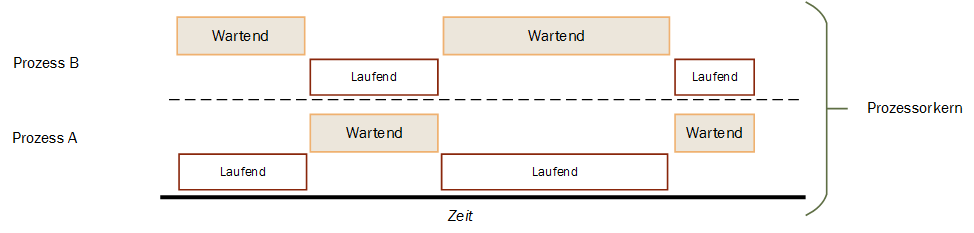
\includegraphics[width=0.7\linewidth]{images/time_slice}
	\caption{Multi-Programmierung\cite[S. 128]{tanenbaum2016}}
	\label{fig:time_slice}
\end{figure}

Einige Arbeitsschritte eines Prozesses können direkt und ohne Verzögerung ausgeführt werden, andere Arbeitsschritte können durch den Zugriff auf langsame Ressourcen wie Festplatten I/O oder Kommunikation über Netzwerke zu Verzögerungen führen. In so einem Arbeitsschritt ist der Prozess blockiert und bis zur Erledigung des Zugriffs kann kein weiterer Arbeitsschritt ausgeführt werden. Das Betriebssystem markiert den Prozess nach dem Start der Anweisung als \emph{blockiert} und wechselt zu einem anderen Prozess. Ein Prozess kann dabei wie in \ref{fig:prozessstati} dargestellt mehrere Stati einnehmen. Er wird im Status Wartend angelegt, wird dann durch das Betriebssystem zur Ausführung ausgewählt und wird damit zum laufenden Prozess. Nach Ablauf der Zeitscheibe\footnote{Oder dem Aufruf einer Betriebssystemmethode wie \textit{yield} oder \textit{sleep} mit der ein thread anzeigen kann dass er nicht mehr weiter aktiv sein möchte} wird die Ausführung des Prozesses unterbrochen und er wird zum wartenden Prozess. Wird während der Ausführung eine Betriebssystemmethode ausgeführt die auf externe Ressourcen wartet dann wird der Prozess unterbrochen und bekommt den Status blockiert. Erst wenn die Betriebssystemmethode abgeschlossen wurde, wird der Prozess in den Status wartend überführt und kann somit wieder zur Ausführung ausgewählt werden.

\begin{figure}
	\centering
	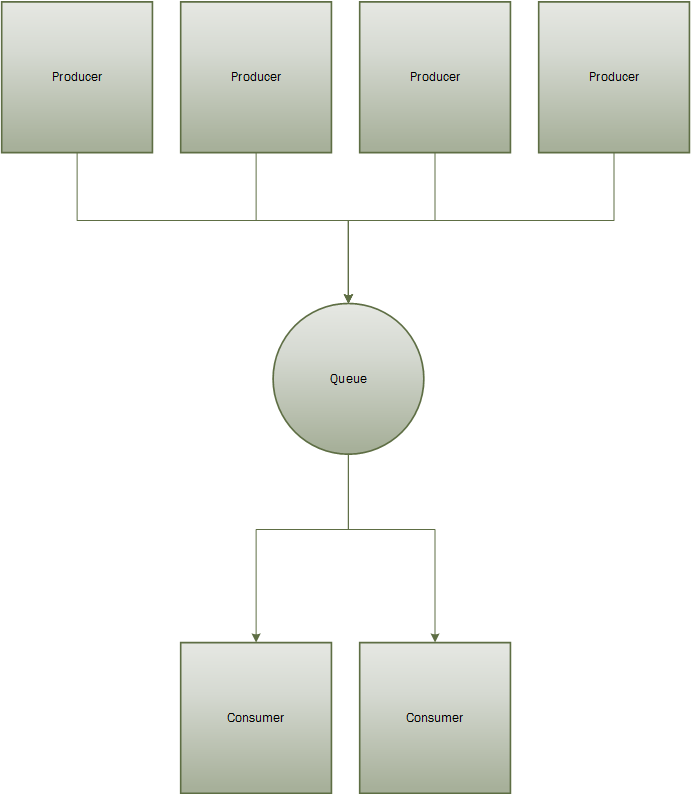
\includegraphics[width=0.7\linewidth]{images/B2_Producer_Consumer_1}
	\caption{Prozessstati\cite[S. 134]{tanenbaum2016}\cite[S. 152]{Dahlin2012}}
	\label{fig:prozessstati}
\end{figure}


Das Betriebssystem wechselt nur zu Prozessen die ausgeführt werden können. Gibt es zu einem Zeitpunkt viele Prozesse die blockiert sind\footnote{meist durch das Warten I/O auf Speichermedien} so ist die I/O Leistung des Rechners der die Leistung begrenzende Faktor, gibt es viele Prozesse die ausgeführt werden könnten ist es die Prozessorleistung.
\\Die lineare Ausführung der Anweisungen kann auch als \emph{thread of control} bezeichnet werden, womit jeder Prozess zumindest einen solchen \emph{thread} hat. Um innerhalb eines Prozesses mehrere Arbeiten gleichzeitig zu erledigen\footnote{Oder auch bestimmte Aufgaben wie I/O einfacher gestalten zu können} kann es wünschenswert sein, mehrere solche threads innerhalb des selben Prozesses, und damit innerhalb eines Adressraums zu verwenden. Dies kann innerhalb eines Prozesses durch die Erzeugung weiterer threads erfolgen. Ein Prozess kann praktisch eine beliebige Anzahl von threads gleichzeitig Anfordern\footnote{Unter Windows beschränkt meist durch den Hauptspeicher, unter Linux durch das Betriebssystem und einstellbar unter \textit{/proc/sys/kernel/threads-max}}. Aus praktischen Gründen sollte die tatsächlich angeforderte Anzahl deutlich darunter liegen, da sonst durch den nötigen Mehraufwand der Verwaltung innerhalb des Betriebssystems die positiven Effekte der Verwendung von threads wieder zunichte gemacht werden\footnote{"[The maximum thread count] doesn't matter, and if you find it does matter, you need to rethink what you're doing so that it doesn't matter"\cite{stacko_threadcount}}.
\\Threads haben \cite[S. 148]{tanenbaum2016}
\begin{itemize}
	\item einen eigenen Befehlszähler, es kann somit jeder thread unabhängig eine eigene Anweisung ausführen.
	\item einen eigenen Stack, und damit eine eigene Aufrufhierarchie und Argumente. für Funktionsaufrufe
	\item eigene Register.
	\item eigenen Zustand( siehe Prozesszustände).
	\item \emph{keinen} eigenen Adressraum, alle threads teilen sich die selben globalen Strukturen wie Dateien oder explizit allokiertem Speicher.
\end{itemize}	
Mit diesen Eigenschaften kann man einen Prozess also vereinfacht auch als einen thread mit Adressraum darstellen.\cite[S. 1]{butenhof1997}
\subsection{Thread Programmierung}
Um threads nutzen zu können stellt das .NET Framework  Methoden zur Verfügung\cite{ms_threading}\footnote{Die Funktionen um mit threads umzugehen folgen meist dem POSIX Thread Standard und sind somit in den meisten Betriebssystemen und Frameworks ähnlich\cite{butenhof1997} }:
\begin{table}[]
	\centering
	\label{Ttab:thread-methoden}
	\begin{tabular}{| l | p{10cm} |}
		\hline
		\textit{\textbf{Methode}} & \textit{\textbf{Beschreibung}}  \\
		\hline
		new Thread()                                         &    Konstruktor mit dem ein neuer Thread angelegt, aber noch nicht gestartet wird\\
		\hline
		Thread.Start/(                                        &    Methode mit der der Thread gestartet wird und mit der Abarbeitung der Thread-Main Methode begonnen wird.\\
		\hline
		Thread.Abort()                                        &   Bricht die Ausführung eines Threads ab\\
		\hline
		Thread.Join()										 & Wartet auf die Beendigung eines Threads\\
		\hline
		Thread.Sleep()										& Unterbricht die Ausführung des Threads für eine bestimmte Zeitspanne\\
		\hline
		Thread.Yield()										& Gibt die Ausführung des aktuellen Threads auf und ermöglicht dem Betriebssystem einen neuen Thread auszuwählen\cite{ms_threading_yield}\\
		\hline
	\end{tabular}
	\caption{.NET thread-Methoden}
\end{table}
Damit kann ein Prozess (und damit der erste thread innerhalb des Prozesses) weitere threads anlegen und diese wieder beenden. Ein einfaches Programm mit mehreren Threads in .NET/ C\# ist in Listing \ref{lst:thread_1} dargestellt.
\begin{lstlisting}[caption={Thread Hello World},label={lst:thread_1},captionpos=b]
class TestThread
{
	private volatile bool runThread = true;
	
	public void Main()
	{
		Thread threadMain = new Thread( ThreadMain );

		threadMain.Start();

		while ( threadMain.IsAlive ) ;

		Thread.Sleep( 10000 );

		runThread = false;
		threadMain.Join();
	}
	
	private void ThreadMain()
	{
		while( runThread )
		{
			Console.Out.WriteLine($"Thread {Thread.CurrentThread.Name} is here");
			Thread.Sleep( 1000 );
		}
	}
}
\end{lstlisting}
In Zeile 7 wird ein neuer Thread angelegt, aber noch nicht gestartet. Das Argument des Konstruktors ist die Methode die beim Starten des threads ausgeführt wird. In Zeile 9 wird der thread gestartet und ist ab diesem Zeitpunkt ausführbar. Die Ausführung startet nicht sofort, sondern dann wen das Betriebssystem den thread zur Ausführung auswählt. Aus diesem Grund wird in Zeile 11 darauf gewartet dass der Thread tatsächlich ausgeführt wurde\footnote{Genau genommen zumindest in einer Zeitscheibe ausgeführt wurde, er kann danach ja wieder unterbrochen werden.}\footnote{Würde man das \textit{Sleep} beginnen ohne dass der thread aktiv geworden ist, könnte die thread-run Variable auf false gesetzt werden, ohne dass der thread auch nur gestartet wurde. Der Zeitpunkt wann der Thread tatsächlich gestartet wird ist nicht vorhersagbar.}.
\\In Zeile 15 wird nach einiger Zeit dem thread mittels tread-run variable mitgeteilt dass er sich beenden soll. Damit kann der thread seine aktuelle Aufgabe beenden und sich danach beenden. Diese Variable muss als \emph{volatile} markiert sein, da sie sich außerhalb des aktuellen threads ändern kann und somit der Zugriff auf den Wert dieser Variable nicht durch Vorhersage der Instruktionen aus dem aktuellen thead vorhergesagt, und damit optimiert werden kann.\cite{ms_volatile} Der thread könnte auch mithilfe von Thread.Abort() abgebrochen werden, dann wird er sofort abgebrochen ohne dass er eine eventuell gerade ausgeführte Aufgabe fertig abarbeiten kann. 
\\In Zeile 16 wird auf die Beendigung des threads gewartet und danach das Programm beendet.


\subsection{Synchronisierung}
Threads sind aus Sicht eines (Applikations-)Entwicklers virtualisierte Prozessorkerne. Der Entwickler kann vereinfacht annehmen dass die Hardware beliebig viele Prozessorkerne hat, die tatsächliche Zuteilung eines threads zur Ausführung auf einen Prozessorkern wird ihm durch das Betriebssystem abgenommen (Siehe Abbildung \ref{fig:threads_cores}). Diese Zuteilung erfolgt für alle threads über Prozessgrenzen hinweg und wird durch viele Parameter beeinflusst\footnote{Insgesamte Auslastung des Rechners, Prioritäten von Threads ...} und ist daher durch den Entwickler nicht vorherzusagen. Der Entwickler darf sich nicht auf eine gewisse Abfolge an Abläufen über mehrere threads hinweg verlassen. Ist eine definierte Reihenfolge notwendig, so muss diese durch den Entwickler explizit erzwungen werden. Die Anzahl an Prozessorkernen im Rechner ist die maximale Anzahl an gleichzeitig aktiven threads.\cite[S. 140]{Dahlin2012}

\begin{figure}
	\centering
	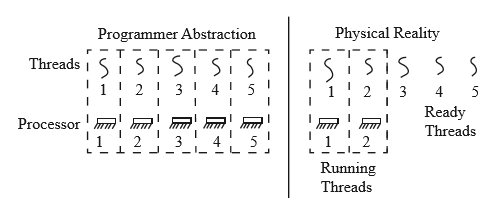
\includegraphics[width=0.7\linewidth]{images/threads_cores.png}
	\caption{Zuteilung threads zu Prozessorkernen\cite[S. 140]{Dahlin2012}}
	\label{fig:threads_cores}
\end{figure}

In fast allen Anwendungszwecken haben threads Daten die nur durch sie selbst verändert werden. Diese werden als \emph{thread-local} oder \emph{per-thread} Daten genannt. Diese Daten können direkt manipuliert werden, da es zu keiner Beeinflussung durch andere threads kommen kann. Diese Daten werden entweder als Variablen am Stack angelegt oder in .NET innerhalb einer Klasse mittels der Hilfsklasse \textit{ThreadLocal} allokiert werden\cite{ms_threadlocal}. 
\\Unglücklicherweise\footnote{Die Formulierung in \cite[S. 179]{Dahlin2012} ist sehr treffend.} besteht aber meist die Notwendigkeit dass threads kooperieren und Daten gemeinsam nutzen müssen. Dies können nun globale Ergebnisdaten einer auf mehrere threads verteilten Berechnung sein oder auch Strukturen zur Verteilung von Arbeit (\textit{dispatching}) auf mehrere threads bei einer Trennung der Erzeugung von Arbeit (producer) und der Erledigung (consumer). Diese Zugriffe von mehreren threads auf dieselben Daten werden auch \emph{race-condition} genannt, da sich die threads ein Rennen liefern wer die Daten zuerst ändern kann.
\\Die einfachste race-condition ist in Codebeispiel \ref{lst:thread_2} dargestellt\cite[S. 182]{Dahlin2012}. Am Ende des Programmes kann nicht mit Sicherheit gesagt werden, welchen Wert die Variable \textit{theValue} hat.

\begin{lstlisting}[caption={Thread race-condition},label={lst:thread_2},captionpos=b]
class TestRaceCondition
{
	private volatile Int32 theValue = 0;
	
	public void Main()
	{
        var thread1 = new Thread( () => theValue = 1 );
		var thread2 = new Thread( () => theValue = 42 );

		thread1.Start();
		thread2.Start();

		thread1.Join();
		thread2.Join();
	}
}
\end{lstlisting}

Solche nicht vorhersagbaren Zustände müssen vermieden werden. Ein erster, naiver Versuch ist in Codebeispiel \ref{lst:thread_3} dargestellt.\cite[S. 180]{Dahlin2012}
\begin{lstlisting}[caption={Thread naiver Mutex},label={lst:thread_3},captionpos=b]
class TestNaiveMutex
{
    private volatile bool stepOneComplete = false;
	private volatile int valueOne = 0;
	private volatile int valueTwo = 0;

	public void Test_NaiveMutex()
	{
		var thread_1 = new Thread( () => {
			valueOne = 42;
			stepOneComplete = true;
		} );

		var thread_2 = new Thread( () => {
			while ( !stepOneComplete ) ;
			valueTwo = valueOne * 2;
		} );

	thread_1.Start(); thread_2.Start();
	thread_1.Join(); thread_2.Join();
}
\end{lstlisting}
Über die Variable \textit{stepOneComplete} wird versucht mit dem zweiten thread so lange zu warten (Zeile 15) bis das Ergebnis des ersten thread vorliegt. Das Problem ist hier nicht offensichtlich, da es erst durch das Kompilieren oder durch die CPU selbst entsteht. Alle modernen Compiler oder CPUs versuchen Code zu optimieren, und eine der Strategien dabei ist das Verschieben von Instruktionen ohne Seiteneffekte innerhalb \textit{eines} threads\cite[S. 100]{ecma335}. Die Verschiebung der Zuweisung in Zeile 11 hätte in einem Programm mit nur einem thread keine Nebenwirkung, diese tritt erst durch den zweiten thread auf, und ist somit durch den Compiler oder die CPU nicht mehr erkennbar.
\\Die beiden obigen Beispiele haben schon in simplen Codebeispielen gezeigt, dass eine korrekte Umsetzung von Zugriffen auf geteilte Datenstrukturen unumgänglich ist. Dafür stehen Entwicklern folgende Methoden zur Verfügung\cite[S. 170ff]{tanenbaum2016}:
\begin{itemize}
	\item Vermeiden von gemeinsamen Datenstrukturen
	\item Atomare Operationen
	\item Speicherbarrieren
	\item Sperren
	\item Monitore
\end{itemize}
\subsubsection{Vermeiden von gemeinsamen Datenstrukturen}	
Das Vermeiden von gemeinsam genutzten Datenstrukturen ist der sicherste und effizienteste Weg um sich vor race-conditions zu schützen. Bei komplexen Aufgaben kann die Stabilität und Ausführungsgeschwindigkeit drastisch erhöht werden wenn die verwendeten Algorithmen - wo möglich - geändert werden, so dass kein Zugriff auf gemeinsame Datenstrukturen notwendig ist. Auch eine Reduktion der Häufigkeit der Zugriffe auf gemeinsam genutzte Datenstrukturen ist hilfreich. So könnten in etwa Ergebnisse innerhalb eines threads berechnet werden und erst am Ende einmalig mit dem Gesamtergebnis zusammengeführt werden, anstatt Ergebnisse einzelner Rechenschritte in ein Gesamtergebnis zu speichern.
\\Diese nicht-globalen Daten können
\begin{enumerate}
	\item in der thread-main Methode allokiert werden und sind damit am Stack der pro thread angelegt wird.
	\item oder als \textit{thread specifc data} deklariert werden. Damit werden diese Datenstrukturen durch die .NET-Runtime für jeden thread extra angelegt.
\end{enumerate}

\subsubsection{Atomare Operationen}	
Eine atomare Operation ist eine Anweisung die durch die CPU ausgeführt wird und in einem Schritt ohne Unterbrechung durchgeführt wird. Diese Operationen beziehen sich auf Datentype mit der Größe der \textit{native word size} des Prozessors\cite[S. 102]{ecma335}, derzeit in der Regel 64bit. In Codebeispiel \ref{lst:thread_2}  in etwa ist der Wert von \textit{theValue} immer 1 oder 42, aber niemals etwas anderes. Würde der Datentyp in etwa \textit{double}\footnote{Double hat eine Länge von 64 bit} sein, ist die Größe des Datentyps nicht mehr atomar, die einfache Zuweisung \textit{theValue = 42;} ist nicht mehr garantiert ohne Unterbrechung durchgeführt zu werden. Somit könnte der erste thread den ersten Teil des Wertes schreiben, dann unterbrochen werden, der zweite thread die Variable setzen, und danach der erste thread den zweiten Teil des Wertes schreiben. Damit ist der Inhalt von \textit{theValue} nicht vorhersagbar. Atomare Operationen sind vor allem für leistungsorientierte Entwicklung wichtig, da sie einen korrekten Zugriff auf zwischen threads geteilte Ressourcen garantieren ohne dass Sperren verwendet werden müssen.
\\In .Net gibt es die eigene Klasse \textit{Interlocked}die mehrere Methoden zur Verfügung stellt die garantiert unterbrechungsfrei sind. Da .Net auf mehreren Plattformen zur Verfügung steht sind diese entweder mittels atomarer Operationen oder mittels Sperren implementiert.

\subsubsection{Speicherbarrieren}
Eine Speicherbarriere ist eine Anweisung an den Compiler und die CPU keine Ablaufoptimierung durch verschieben von Instruktionen über die Barriere hinweg durchzuführen. Es wird also garantiert dass alle Anweisungen vor der Barriere von der CPU tatsächlich vor allen anderen Anweisungen nach der Barriere ausgeführt werden.\cite[S. 195]{tanenbaum2016} Damit kann das in Codebeispiel \ref{lst:thread_3} angeführte Problem behoben werden. In C\# wird eine Speicherbarriere durch den Aufruf von \textit{Interlocked.MemoryBarrier()} realisiert.\cite{ms_interlocked_barrier}\footnote{Siehe auch \textit{NaiveMutexBarrier.cs}}

\subsubsection{Sperren}	
Sperren (locks) bieten eine Möglichkeit sicherzustellen dass nur ein thread innerhalb eines bestimmten Abschnittes des Codes aktiv sein kann. Die Ausführung aller Anweisungen innerhalb des mit einer Sperre geschützten Bereiches wirken auf alle anderen threads \textit{atomar} da immer alle Anweisungen ausgeführt werden bevor ein anderer thread den Code-Block ausführen kann. Dadurch können Veränderungen an Datentypen die nicht atomar sind durchgeführt werden und ein konsistenter Zustand der Daten garantiert werden. 
\\Die Ausführung von Code innerhalb einer Sperre kann natürlich weiterhin unterbrochen werden und zu einem späteren Zeitpunkt fortgesetzt wird. Versucht ein anderer thread die selbe Sperre für sich zu allokieren, wird der thread unterbrochen und in den Status blockiert gesetzt. Erst wenn die Sperre durch den ersten thread freigegeben wird, setzt das Betriebssystem den thread in den Status wartend. Dadurch steht er für die Ausführung innerhalb einer der nächsten Zeitscheiben bereit. Auch hier gilt, dass der zweite thread nicht sofort nach frei werden der Sperre ausgeführt wird, sondern zu einem beliebigem Zeitpunkt.

\subsubsection{Monitore}	
Mit den bisher vorgestellten Techniken kann ein Programm mit mehreren threads korrekt, also ohne unbeabsichtigte Seiteneffekte durch Manipulation von globalen Daten\footnote{Daten die für mehrere threads sichtbar sind.}  implementiert werden. 
\\Monitore\footnote{Oder auch \textit{condition} genannt\cite[S. 199]{Dahlin2012}.} bieten die Möglichkeit, dass ein thread auf einen anderen thread wartet. Dies wird in benötigt, wenn ein thread für die Abhandlung der Kommunikation zuständig ist (der sogenannte Erzeuger), und ein anderer thread die Abarbeitung der übermittelten Dateninhalte durchführt (der so genannte Verbraucher). Nur mit den bisher vorgestellten Methoden ist dies nur mittels \textit{polling}, einem ständigen Nachfragen durch den zweiten thread, möglich\footnote{Dies wird Erzeuger-Verbraucher (producer-consumer) Problem genannt\cite[S. 188]{tanenbaum2016}}\cite[S. 199ff]{Dahlin2012}. 
\begin{lstlisting}[caption={Thread naiver Monitor},label={lst:thread_busywait},captionpos=b]
public T DequeBusy()
{
	bool dequeSuccess = false;
	T result = default( T );

	while ( !dequeSuccess )
	{
		lock ( myLock )
		{
			if( backingStore.Any() )
			{
				dequeSuccess = true;
				return backingStore.Dequeue();
			}
		}
	}
}

\end{lstlisting}
Diese Implementierung, wie in Codebeispiel \ref{lst:thread_busywait} dargestellt, hat den gravierenden Nachteil dass der thread Rechenleistung verbraucht ohne tatsächliche Arbeit zu verrichten. Dies geschieht durch die Schleife in Zeile 6, die erst verlassen wird wenn tatsächlich wieder Arbeit vorhanden ist. Damit kann dieser eine thread sogar die Ausführung der weiteren threads, also auch des threads der die Arbeit erzeugt, verlangsamen. Das Hinzufügen eines \textit{sleep} Befehls oder eines erzwungenen thread-Wechsel mittels \textit{yield} mildert zwar das Problem der CPU-Belastung, jedoch führen beide Instruktionen zu einem Overhead da die threads in kurzer Zeit gewechselt werden müssen, was auch zu einer hohen CPU Beanspruchung führt.
\\Monitore bieten nun die Möglichkeit zusammen mit Sperren dies zu lösen. Dazu stellen sie folgende Methoden zur Verfügung:\cite[S. 201]{Dahlin2012}\cite{ms_monitor}
\begin{itemize}
	\item \textit{Wait()} - Gibt in einem atomaren Schritt die verbundene Sperre frei und versetzt den thread in den Status blockiert. Damit wird der thread nicht weiter ausgeführt und verbraucht keine CPU-Ressourcen mehr. Der thread wird in der Monitor-Variable als auf diese wartend eingetragen\footnote{in .Net ist dies die Sperrvariable.}. Vor der Rückkehr aus der Methode wird die Sperre wieder gesetzt.
	\item \textit{Signal()} (in .Net \textit{Pulse()} genannt) - Setzt einen der auf diese Monitor -Variable wartenden threads in den Zustand Wartend, damit wird er gemäß dem Scheduling ausgeführt\footnote{Die Ausführung beginnt nicht sofort, der Zeitpunkt ist abhängig von der Last im System}.
	\item \textit{Broadcast()} (in .Net \textit{PulseAll()} genannt) - Setzt alle threads die auf diese Monitor-Variable warten in den Zustand Wartend. Damit werden alle diese threads ausgeführt.
\end{itemize}
 Damit kann das Codebeispiel \ref{lst:thread_busywait} nun korrekt umgesetzt werden, wie in Codebeispiel\ref{lst:thread_deq} dargestellt.
\begin{lstlisting}[caption={Thread Monitor.Wait()},label={lst:thread_deq},captionpos=b]
public T Dequeue()
{
	lock( myLock )
	{

		while ( ! backingStore.Any() )
		{
			Monitor.Wait( myLock );
		}

		return backingStore.Dequeue();
	}
}
\end{lstlisting}
In Zeile 8 wird der thread solange unterbrochen bis der Monitor von einem anderen thread signalisiert wird. Die Sperre ist vor dem Eintritt in das Wait() gesetzt. Die Schleife in Zeile 6 hat mehrere Aufgaben. Wenn schon Arbeit existiert, wird diese ohne weiteres Wait() abgearbeitet. Dies ist notwendig, da ein vorhergehendes \textit{Pulse} nicht auf der Monitor-Variable vermerkt wird. Würde also Wait() ohne Prüfung aufgerufen werden, so würde der thread unterbrochen werden obwohl Arbeit vorhanden wäre. Desweiteren wird nachdem \textit{Wait()} verlassen wird wieder geprüft ob tatsächlich Arbeit vorhanden ist. Dies ist notwendig, denn wenn es mehrere Verbraucher gibt kann die von einem anderen thread erzeugte Arbeit bereits durch einen anderen thread abgearbeitet sein. Der dann durch das \textit{Pulse()} aufgeweckte thread findet dann keine weitere Arbeit mehr vor. Dies ist in Ablaufdiagram \ref{fig:threads_pcs} dargestellt.

\begin{figure}
	\centering
	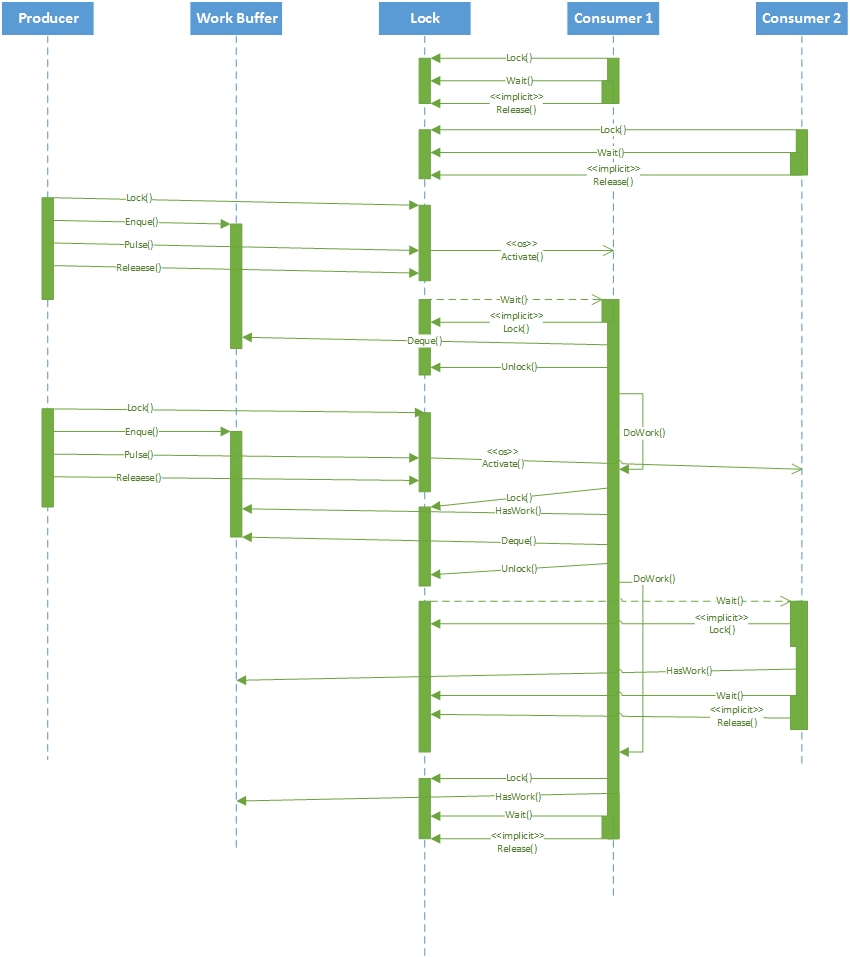
\includegraphics[width=0.9\linewidth]{images/uml-sequence_pulse.png}
	\caption{Erzeuger/ Verbraucher Modell - Ablauf \cite[S. 405]{posa2} }
	\label{fig:threads_pcs}
\end{figure}

Der Erzeuger ist in Codebeispiel \ref{lst:thread_enq} dargestellt. Nachdem die Sperre gesetzt wird, wird die neue Arbeit in Zeile 5 eingetragen und in Zeile 7 wird die Monitor-Variable ausgelöst, was zu einer - zeitlich verzögerten - Aktivierung eines Verbraucher-threads führt. Die Sperre wird während des Aufrufes von \textit{Pulse()} nicht modifiziert, sie bleibt erhalten.
\begin{lstlisting}[caption={Thread Monitor.Pulse()},label={lst:thread_enq},captionpos=b]
public void Enque( T newElement )
{
	lock( myLock )
	{
		backingStore.Enqueue( newElement );

		Monitor.Pulse( myLock );
	}
}
\end{lstlisting}
\subsection{Zusammenfassung}
Threads stellen eine wichtigen Baustein der Programmierung dar, vor allem wen es darum geht performante Programme zu entwickeln die komplexe Aufgabenstellungen zu bewältigen haben. Threads werden oft von eingesetzten Frameworks verwendet und vom Entwickler versteckt, daher ist ein Grundwissen für alle Entwickler notwendig. 
\\Die essentiellen Punkte wenn es um Concurrency geht sind
\begin{itemize}
	\item sich dessen bewusst zu sein welche Daten global, also für mehrere threads sichtbar sind, und wie diese zu schützen sind. 
	\item sich bewusst zu sein, dass es keine Garantien für Zeitpunkte gibt. Jeder thread kann zu jedem Zeitpunkt, auch innerhalb einer Sperre, unterbrochen werden und erst zu einem späteren, nicht vorhersehbarem Zeitpunkt fortgesetzt werden.
	\item zu wissen, das das Starten oder Aufwecken eines threads nicht sofort erfolgt, sonder auch erst zu einem späterem, durch das Betriebssystem festgelegten Zeitpunkt.
\end{itemize}


\section{Relationale Datenbanken}
Datenbanken sind Systeme in denen große Datenmengen effizient gespeichert und verwaltet werden können. Dabei wird vom System eine Schnittstelle zur Verfügung gestellt die das Arbeiten mit den Daten ohne Wissen über deren tatsächliche Speicherung ermöglicht. Die Daten innerhalb des Systems werden in einem \emph{Modell} beschrieben, das die Komplexität der physischen Speicherung nicht darstellt. Diese bleibt dem System selbst überlassen und wird von diesem bei den meisten modernen Systemen dynamisch ausgewählt um für die jeweiligen Daten und die Art der Zugriffe auf diese eine optimale Leistung zur Verfügung zu stellen.
\\CITATION NEEDED
\\Bei relationalen Datenbanken werden die Informationen nach thematischer Zusammengehörigkeit in so genanten Tabellen gespeichert.\footnote{\emph{Relational} wird in seiner mathematischen Bedeutung verwendet.} Diese Art von Datenbanken wurde erstmals von Edgar F. Codd vorgestellt und galt bis vor wenigen Jahren als alleiniger Standard für Datenbanken. \cite[S. 133]{dbgrund}. Erst durch die immensen Datenmengen der Big-Data wurde für diese Anwendung die so genannten \emph{No-SQL}\footnote{\emph{N}ot \emph{O}nly \emph{SQL}, diese Datenbanken stellen weitere Formen der Speicherung wie schemenlose Dokument-Datenbanken, Wertepaare oder Graphdatenbanken zur Verfügung. CITATION } Datenbanken eingeführt. Bei diesen werden einige der unten Beschriebenen strengen Regeln der Datenstruktur und Datenkonsistenz aufgehoben um eine höhere Leistung zu erreichen.
\\Bei relationalen Datenbanken werden thematisch Zusammengehörige Daten in einer Tabelle gespeichert. Jede Datenbank umfasst mehrerer solcher Tabellen. Jede Tabelle enthält Datensätze, so genannte \emph{Tupel}. Jeder dieser Tupel besteht aus immer den selben \emph{Attributen}, die beschreiben welche Daten die Tabelle enthält. Tabellen sind also eine Zusammensetzung aus der Beschreibung der Struktur der Daten und den Daten selbst. Die Beschreibung der Struktur der Daten wird auch \emph{Schema} oder \emph{Katalog} genannt.
\\Ein Beispiel für eine Tabelle ist die Tabelle 'Student', die die Attribute Vorname, Nachname, Matrikelnummer und Geburtsjahr enthält. Ein Datensatz darin ist dann zum Beispiel 'Max', 'Mustermann', '4711', '1980'.\cite[S. 137]{dbgrund} \cite{DBLP:journals/cacm/Codd70}
\\Die von Codd vorgeschlagene Trennung in Benutzersicht und Speicherung hat nun den Vorteil dass der Student (Vorname: 'Max', Nachname: 'Mustermann') durch Änderung der Beschreibung der Sicht auch als Student( Nachname: 'Mustermann', Geburtsjahr: '1980') dargestellt werden kann.\footnote{Dies wird auch \emph{Projektion} genannt, eine Änderung der Darstellung ohne Änderung der zugrundeliegenden Daten\cite[S. 152]{dbgrund} }
\\Bei relationalen Datenbanken hat sich als Standard für die Manipulation des Schemas und der Daten die SQL\footnote{\emph{S}tructured \emph{[Q}uery \emph{L}anguage, genormt nach der ISO/ IEC 19075 Standard-Familie der von allen relationalen Datenbanksystemen unterstützt wird\cite{ocl_sql}\cite{isosql}\footnote{Jeweils mit eigenen, unterschiedlich mächtigen Erweiterungen um den Anwendungsentwicklern einen Austausch des zugrundeliegenden Systems zu erschweren}} etabliert. Mit deren Hilfe können\cite[S. 182]{dbgrund}
\begin{itemize}
	\item Schemata verwaltet werden. Dieser Teil der Sprache wird auch \emph{Data Manipulation Language (DML)} genannt. Er enthält Befehle um 
	\begin{itemize}
		\item Tabellen anzulegen
		\item Tabellen zu modifizieren
		\item Tabellen zu löschen und
		\item Beschränkungen anzulegen und zu löschen.
	\end{itemize}
	\item Daten verwaltet werden. Dieser Teil der Teil der Sprache wird auch \emph{Data Definition Language (DDL)} genannt. Er enthält Befehle um
	\begin{itemize}
		\item Datensätze anzulegen
		\item Datensätze auszulesen
		\item Datensätze zu modifizieren und
		\item Datensätze zu löschen.
	\end{itemize}
\end{itemize} werden.
Zusätzlich zu dieser Standardisierung des Zugriffes bieten relationale Datenbanksysteme weitere Garantien die das Arbeiten mit großen Datenmengen vereinfachen. Diese Garantien beziehen sich auf Veränderungen von Daten die in so genannten \emph{Transaktionen} durchgeführt werden. Eine Transaktion beinhält dabei alle Veränderungen an Daten die als Einheit durchgeführt werden sollen. Entweder werden alle Veränderungen erfolgreich durchgeführt, oder aber keine einzige der Veränderungen innerhalb einer Transaktion wird durchgeführt. Diese Garantien werden auch als \emph{ACID} bezeichnet:\cite[S. 6fs]{GrayReuter93}
\begin{itemize}
	\item \emph{Atomic} (Atomar) - Die Veränderungen die eine Transaktion am Datenbestand durchführt sind atomar, sie werden also alle durchgeführt oder keine der Veränderungen findet statt.
	\item \emph{Consistent} (Konsistent) - Die Transaktion ist eine innerhalb der im Schema definierten Regeln gültige Veränderung der Daten. Die Daten sind am Ende der Transaktion in einem gültigen und konsistenten Zustand.
	\item \emph{Isolated} (Isoliert) - Transaktionen laufen unabhängig voneinander ab, obwohl sie zeitgleich laufen können. Eine zweite Transaktion findet entweder komplett vor oder komplett nach einer Transaktion statt.
	\item \emph{Durable} (Dauerhaft) - Wenn eine Transaktion erfolgreich abgeschlossen wurde, ist die Veränderung dauerhaft gespeichert, auch wenn es danach zu Fehlern oder Abstürzen kommt.
\end{itemize}
\subsection{Sperren}
asdas
\subsection{Isolationsebenen}
sdfsdf

\chapterend
